\documentclass[aspectratio=169, 11pt]{beamer}

% ====== Theme ======
\usetheme{Madrid}
\definecolor{CityUBlue}{RGB}{0, 51, 102}
\definecolor{CityULightBlue}{RGB}{0, 102, 179}
\definecolor{CityUGold}{RGB}{198, 163, 0}
\usecolortheme[named=CityUBlue]{structure}
\setbeamercolor{title}{fg=white, bg=CityUBlue}
\setbeamercolor{frametitle}{fg=white, bg=CityUBlue}
\setbeamercolor{block title}{bg=CityUBlue, fg=white}
\setbeamercolor{block body}{bg=CityUBlue!10, fg=black}
\setbeamercolor{item}{fg=CityUBlue}
\setbeamercolor{subitem}{fg=CityULightBlue}

% ====== Packages ======
\usepackage[T1]{fontenc}
\usepackage{lmodern}
\usepackage{booktabs}
\usepackage{graphicx}
\usepackage{hyperref}
\usepackage{amsmath, amssymb}
\usepackage{tikz}
\usepackage{appendixnumberbeamer}

% ====== Settings ======
\setbeamertemplate{navigation symbols}{}
\graphicspath{{figures/}{../../Figures used in slides/}}

% ====== Metadata ======
\title[EF8083 Lecture 3]{PhD Lecture in Behavioral Asset Pricing:\\ Preferences \& Beliefs (I)}
\author[F.\ W.\ Li]{Frank Weikai Li}
\institute[CityU]{Associate Professor of Finance\\City University of Hong Kong}
\date{}

% ==============================================================================
\begin{document}
% ==============================================================================

% --- Slide 1: Title ---
\begin{frame}[plain]
\titlepage
\end{frame}

% --- Slide 2: Overview ---
\section{Overview}

\begin{frame}{Overview}
\begin{itemize}
\item To derive the predictions of irrationality, we usually need to make more assumptions about the form of irrationality
  \begin{itemize}
  \item One source of guidance is the psychology literature
  \end{itemize}
\item The rational benchmark has two elements:
  \begin{itemize}
  \item When agents receive new information, they update their beliefs correctly (according to Bayes' rule)
  \item Given their beliefs, agents make sensible decisions (according to Expected Utility)
  \end{itemize}
\item We draw primarily on two strands of the psychology literature
  \begin{itemize}
  \item Psychology of preferences (deviations from EU)
  \item Psychology of beliefs (deviations from Bayes' rule)
  \end{itemize}
\end{itemize}
\end{frame}

% --- Slide 3: Roadmap ---
\begin{frame}{Roadmap}
\begin{itemize}
\item \textbf{Psychology of preferences:}
  \begin{itemize}
  \item Prospect theory (risk preferences when probabilities are objectively known)
  \item Ambiguity aversion (risk preferences when probabilities are not objectively known)
  \end{itemize}
\item \textbf{Psychology of beliefs:}
  \begin{itemize}
  \item Representativeness, overconfidence, over-extrapolation, belief perseverance/confirmation bias, anchoring, availability
  \end{itemize}
\item \textbf{How ``feelings'' affect preferences and beliefs}
  \begin{itemize}
  \item Affective feelings, cognitive feelings
  \end{itemize}
\item \textbf{Models of heterogeneous beliefs}
\end{itemize}
\end{frame}

% --- Slide 4: Prospect Theory ---
\section{Prospect Theory}

\begin{frame}[shrink=5]{Prospect Theory}
\begin{itemize}
\item Most models of financial markets assume that investors evaluate risk according to Expected Utility (EU)
  \begin{itemize}
  \item Utility function that is increasing, concave, and defined over consumption outcomes
  \end{itemize}
\item However, a large body of work shows that, at least in experimental settings, EU is not an accurate description of risk attitudes
\item Many non-EU models that try to capture these departures from EU
  \begin{itemize}
  \item Prospect theory, due to Kahneman and Tversky (1979, 1992), is the best-known example
  \end{itemize}
\item This is a `descriptive' theory of behavior:
  \begin{itemize}
  \item How we actually behave, not how we \emph{should} behave
  \end{itemize}
\item \textbf{Prospect theory has four key features:}
  \begin{itemize}
  \item Reference Dependence
  \item Loss Aversion
  \item Probability Weighting
  \item Risk aversion over gains, risk seeking over losses (diminishing sensitivity)
  \end{itemize}
\end{itemize}
\end{frame}

% --- Slide 5: Reference Dependence ---
\begin{frame}{Reference Dependence}
\begin{itemize}
\item The carriers of utility are gains and losses relative to some reference point, not final wealth levels
  \begin{itemize}
  \item Experimental evidence
  \item Introspection
  \item Consistent with perception of other attributes
  \end{itemize}
\item We are more sensitive to changes in brightness, loudness, or temperature than to absolute levels of these attributes
  \begin{itemize}
  \item E.g., put two hands in separate basins of hot and cold water, then in one large warm bath
    \begin{itemize}
    \item The hot hand feels the water as colder than the cold hand does!
    \end{itemize}
  \end{itemize}
\end{itemize}
\end{frame}

% --- Slide 6: Loss Aversion ---
\begin{frame}{Loss Aversion}
\centering
\href{https://www.youtube.com/watch?v=vBX-KulgJ1o}{Loss aversion -- video demo}
\end{frame}

% --- Slide 7: Loss Aversion, ctd. ---
\begin{frame}{Loss Aversion, ctd.}
\begin{columns}[T]
\begin{column}{0.50\textwidth}
\begin{itemize}
\item It turns out that we dislike losses roughly twice as much as we like equal-sized gains
\item We hate losing
\end{itemize}
\end{column}
\begin{column}{0.48\textwidth}
\centering
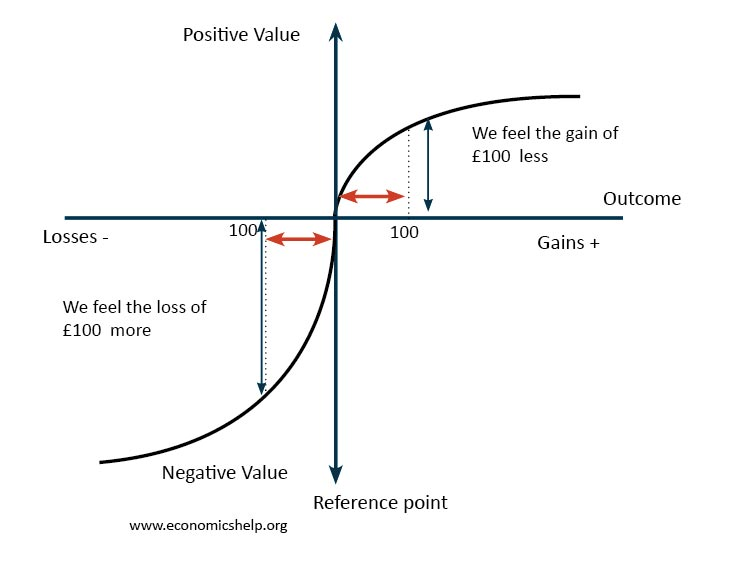
\includegraphics[width=\textwidth]{figures/slide07_pic1.jpg}
\end{column}
\end{columns}
\end{frame}

% --- Slide 8: Probability Weighting ---
\begin{frame}{Probability Weighting}
\vfill
\centering

\includegraphics[width=0.6\textwidth]{figures/slide08_pic1.png}
\vfill
\end{frame}

% --- Slide 9: Probability Weighting, ctd. ---
\begin{frame}{Probability Weighting, ctd.}
\begin{itemize}
\item Many of us -- simultaneously -- buy lottery tickets and insurance
\item Buying lottery tickets means that people prefer a 1 in 1000 chance of winning \$5000 to a certain \$5
  \begin{itemize}
  \item $(\$5, 1) \prec (\$5000, 0.001)$
  \end{itemize}
\item Buying insurance means that people prefer to pay \$5 rather than to face a 1 in 1000 chance of losing \$5000
  \begin{itemize}
  \item $(-\$5000, 0.001) \prec (-\$5, 1)$
  \end{itemize}
\item Difficult to explain under Expected Utility: risk aversion and risk seeking at the same time
\item \textbf{Probability weighting:} people overweight low probability events
\end{itemize}
\end{frame}

% --- Slide 10: Probability Weighting, ctd. ---
\begin{frame}{Probability Weighting, ctd.}
\begin{columns}[T]
\begin{column}{0.55\textwidth}
\begin{itemize}
\item Overweight small probability events
\item \textbf{What is the psychological foundation?}
\item Could come from salience
  \begin{itemize}
  \item We find it difficult to assess probabilities
  \item In our mind's ``model'' we often solve the problem by recalling things from the past
  \item How easy we find it to recall the related incident is our mind's simple proxy for how likely the event is to occur
  \end{itemize}
\end{itemize}
\end{column}
\begin{column}{0.43\textwidth}
\centering
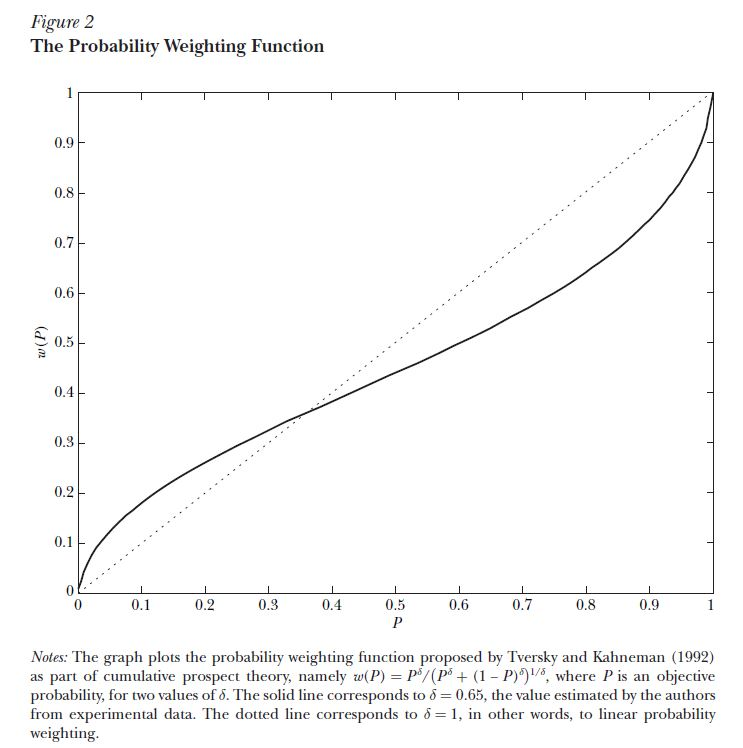
\includegraphics[width=\textwidth]{figures/slide10_pic1.jpg}
\end{column}
\end{columns}
\end{frame}

% --- Slide 11: Prospect Theory Framework ---
\begin{frame}{Putting It All Together: Prospect Theory}
\begin{itemize}
\item \textbf{``Prospect Theory''}
\item The original version (Kahneman and Tversky, 1979) considers the gamble $(x, p; y, q)$
\item Under EU, it is assigned the value:
\[
p \cdot U(W + x) + q \cdot U(W + y)
\]
\item So, accept the lottery if $p \cdot U(W + x) + q \cdot U(W + y) > U(W)$
\item Under prospect theory, it is assigned the value:
\[
w(p) \cdot v(x) + w(q) \cdot v(y)
\]
\item So, accept the lottery if $w(p) \cdot v(x) + w(q) \cdot v(y) > v(0)$
\end{itemize}
\end{frame}

% --- Slide 12: Prospect Theory Features ---
\begin{frame}{Prospect Theory, ctd.}
\textbf{Four key features:}
\begin{enumerate}
\item \textbf{Reference dependence}
  \begin{itemize}
  \item The carriers of value are gains and losses, not final wealth levels ($x$ \& $y$, not $W+x$ \& $W+y$)
  \end{itemize}
\end{enumerate}
\end{frame}

% --- Slide 13: Loss Aversion Feature ---
\begin{frame}{Prospect Theory, ctd.}
\begin{columns}[T]
\begin{column}{0.55\textwidth}
\begin{enumerate}
\setcounter{enumi}{1}
\item \textbf{Loss aversion}
  \begin{itemize}
  \item $v(\cdot)$ is the value function, and it has a kink at the origin
  \item Captures a greater sensitivity to losses (even small losses) than to gains of the same magnitude
  \item Inferred from aversion to $(\$110, 1/2; -\$100, 1/2)$
  \item An Expected Utility individual is almost risk-neutral over small-stakes gambles
  \end{itemize}
\end{enumerate}
\end{column}
\begin{column}{0.43\textwidth}
\centering
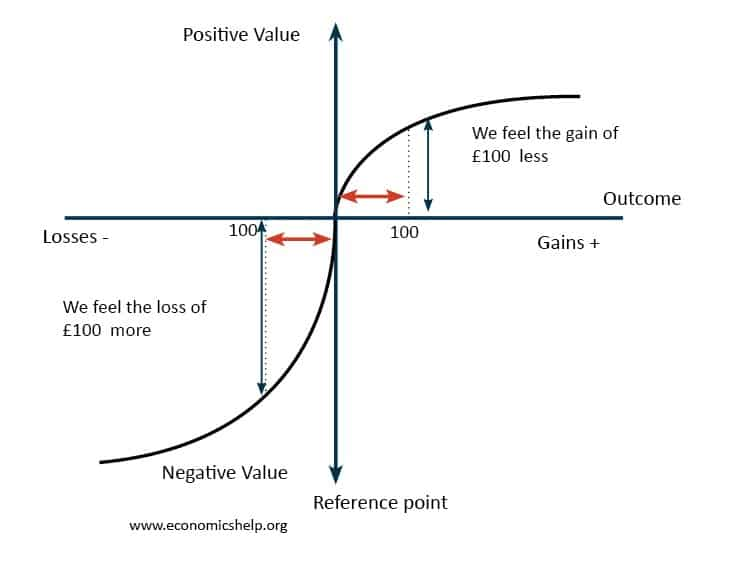
\includegraphics[width=\textwidth]{figures/value_function.jpg}
\end{column}
\end{columns}
\end{frame}

% --- Slide 14: Probability Weighting Feature ---
\begin{frame}{Prospect Theory, ctd.}
\begin{enumerate}
\setcounter{enumi}{2}
\item \textbf{Probability weighting}
  \begin{itemize}
  \item Transform probabilities with a weighting function $w(\cdot)$ that overweights low probabilities
  \item Inferred from our simultaneous liking of lotteries and insurance, e.g., $(\$5, 1) \prec (\$5000, 0.001)$ and $(-\$5000, 0.001) \prec (-\$5, 1)$
  \item Transformed probabilities should not be thought of as erroneous beliefs, but as decision weights
  \item Could come from: evolution / salience
  \end{itemize}
\end{enumerate}
\end{frame}

% --- Slide 15: Risk Preferences Feature ---
\begin{frame}{Prospect Theory, ctd.}
\begin{enumerate}
\setcounter{enumi}{3}
\item \textbf{Risk aversion over gains, risk seeking over losses}
  \begin{itemize}
  \item $v(\cdot)$ is concave over gains, convex over losses
  \item i.e., people want to avoid risk \& lock in gains when they have made money (``concave over gains'')
  \item But are more willing to hold on to gambles and take risk when they have lost money on them (``convex over losses'')
  \item Inferred from $(\$500, 1) \succ (\$1000, 1/2; \$0, 1/2)$ and $(-\$500, 1) \prec (-\$1000, 1/2; \$0, 1/2)$
  \end{itemize}
\end{enumerate}
\end{frame}

% --- Slide 16: Risk Preferences Graph ---
\begin{frame}{Prospect Theory, ctd.}
\begin{columns}[T]
\begin{column}{0.50\textwidth}
\begin{itemize}
\item Risk aversion over gains, risk seeking over losses
\item Prefer more volatile stocks in the domain of capital losses
\item Prefer less volatile stocks in the domain of capital gains
\end{itemize}
\end{column}
\begin{column}{0.48\textwidth}
\centering
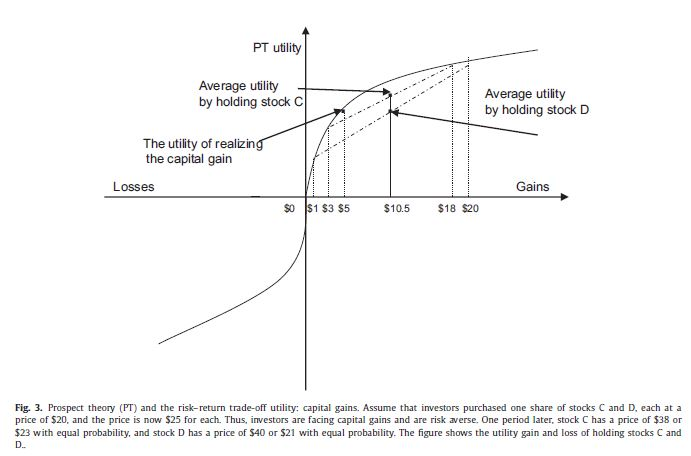
\includegraphics[width=\textwidth]{figures/slide16_pic1.jpg}
\end{column}
\end{columns}
\end{frame}

% --- Slide 17: Four-fold Pattern ---
\begin{frame}{Prospect Theory, ctd.}
\begin{itemize}
\item Prospect theory captures a ``four-fold pattern'' of risk attitudes:
  \begin{itemize}
  \item Risk aversion over moderate-probability gains
  \item Risk seeking over moderate-probability losses
  \item Risk seeking over low-probability gains
  \item Risk aversion over low-probability losses
  \end{itemize}
\item Having preferences different from standard rational theory is not a `mistake'
\end{itemize}
\end{frame}

% --- Slide 18: Narrow Framing ---
\section{Narrow Framing}

\begin{frame}[shrink=5]{Narrow Framing}
\begin{itemize}
\item \textbf{Key question:} what should the argument of $v(\cdot)$ be?
  \begin{itemize}
  \item This is a question about ``framing''
  \end{itemize}
\item In a traditional model where utility is defined over total wealth or lifetime consumption, the agent evaluates a new risk by combining it with pre-existing risks and checking whether the combination is an improvement
\item But in experimental settings, people often seem to evaluate a new risk in isolation, separately from other concurrent risks
  \begin{itemize}
  \item ``narrow framing''
  \item E.g., the widespread rejection of the gamble $(\$110, 1/2; -\$100, 1/2)$ is not only evidence of loss aversion, but of narrow framing as well
  \end{itemize}
\item \textbf{Where does narrow framing come from?}
  \begin{itemize}
  \item A heuristic used to simplify complex decisions
  \item Difficult for an individual to compute the distribution of gains and losses in overall wealth
  \end{itemize}
\end{itemize}
\end{frame}

% --- Slide 19: Applications Overview ---
\section{Prospect Theory Applications}

\begin{frame}{Prospect Theory Applications}
\begin{itemize}
\item \textbf{Trading Behavior}
  \begin{itemize}
  \item Try to address the disposition effect and other trading phenomena
  \item All aspects of prospect theory play a role
  \end{itemize}
\item \textbf{The cross-section of stock returns}
  \begin{itemize}
  \item Try to address the high-risk--low-alpha and momentum/PEAD puzzles
  \item New prediction: the pricing of skewness
  \item Probability weighting and diminishing sensitivity play a central role
  \end{itemize}
\item \textbf{The aggregate stock market}
  \begin{itemize}
  \item Try to address the equity premium, non-participation, excess volatility, and predictability puzzles
  \item Loss aversion plays a key role
  \item But probability weighting also matters
  \end{itemize}
\end{itemize}
\end{frame}

% --- Slide 20: Investor Trading Behavior ---
\section{Investor Trading Behavior}

\begin{frame}{Investor Trading Behavior}
\begin{itemize}
\item Prospect theory can explain the disposition effect
  \begin{itemize}
  \item Investors' tendency to hold on to losers and sell winners too quickly
  \end{itemize}
\end{itemize}
\vfill
\centering
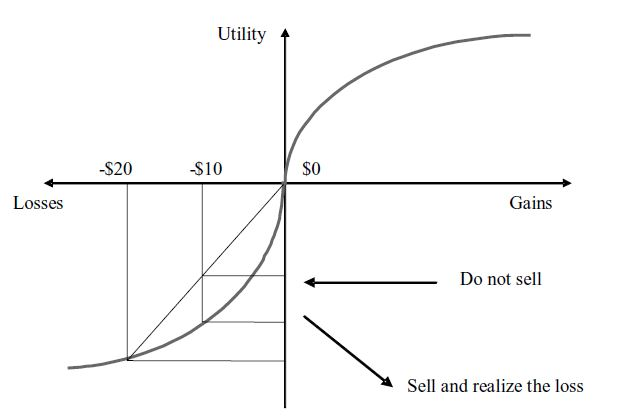
\includegraphics[width=0.45\textwidth]{figures/slide20_pic1.jpg}
\hspace{0.5em}
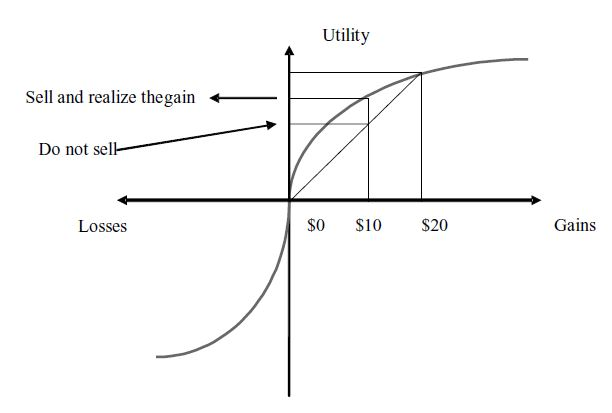
\includegraphics[width=0.45\textwidth]{figures/slide20_pic2.jpg}
\end{frame}

% --- Slide 21: The Cross-section ---
\section{The Cross-Section of Stock Returns}

\begin{frame}[shrink=5]{The Cross-Section}
\textbf{Barberis and Huang (AER 2008), Stocks as Lotteries\ldots}
\begin{itemize}
\item Single period model
\item A risk-free asset and $J$ risky assets with multivariate Normal payoffs
\item Agents have identical expectations about security payoffs
\item Agents have identical cumulative prospect theory preferences
\end{itemize}
\vspace{0.5em}
\textbf{Now introduce a small, independent, positively skewed security into the economy:}
\begin{itemize}
\item Obtain a novel prediction: the new security earns a negative excess return
\item Skewness itself is priced, in contrast to the EU model where only coskewness with the market matters
\end{itemize}
\vspace{0.5em}
\textbf{Equilibrium involves heterogeneous holdings:}
\begin{itemize}
\item Some investors hold a large, undiversified position in the new security
\item Others hold no position in it at all
\item Since the new security contributes skewness to the portfolios of some investors, it is valuable, and so earns a low average return
\end{itemize}
\end{frame}

% --- Slide 22: Cross-section, ctd. ---
\begin{frame}{The Cross-Section, ctd.}
\begin{columns}[T]
\begin{column}{0.55\textwidth}
\begin{itemize}
\item When investors increase their allocation to lottery stocks, they lose diversification benefits
\item But when the allocation gets larger, the positive idiosyncratic skewness outweighs the loss of diversification
\end{itemize}
\end{column}
\begin{column}{0.42\textwidth}
\centering
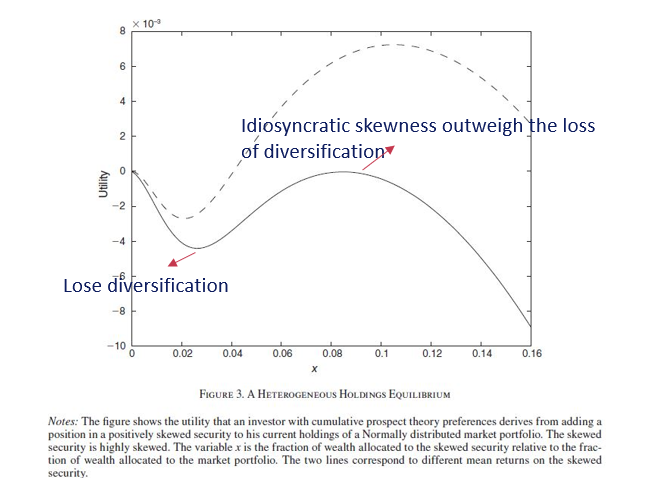
\includegraphics[width=\textwidth]{figures/22.png}\\
\footnotesize Barberis and Huang (2008)
\end{column}
\end{columns}
\end{frame}

% --- Slide 23: IPO Application ---
\begin{frame}{The Cross-Section, ctd.}
\begin{columns}[T]
\begin{column}{0.55\textwidth}
\textbf{Applications:}
\begin{itemize}
\item Low long-run return on IPOs
  \begin{itemize}
  \item IPO returns are highly positively skewed: Google, Microsoft, Walmart\ldots
  \item Green and Hwang (2012): IPOs predicted to be more positively skewed have higher first-day returns and lower long-run returns
  \end{itemize}
\end{itemize}
\end{column}
\begin{column}{0.42\textwidth}
\centering
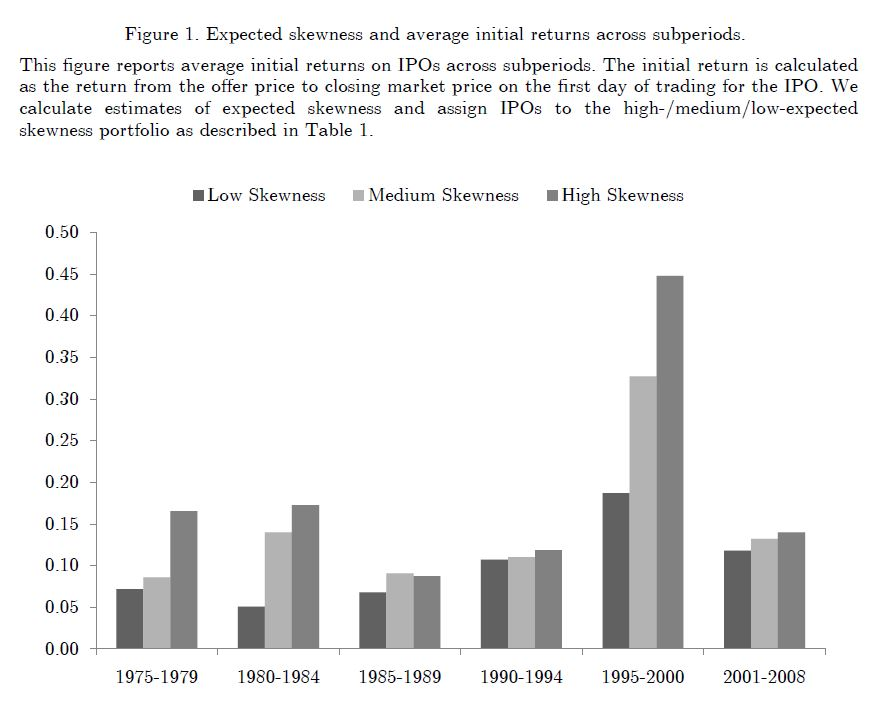
\includegraphics[width=\textwidth]{figures/slide23_pic1.jpg}
\end{column}
\end{columns}
\end{frame}

% --- Slide 24: More Applications ---
\begin{frame}[shrink=5]{The Cross-Section, ctd.}
\begin{columns}[T]
\begin{column}{0.55\textwidth}
\textbf{Applications, ctd.}
\begin{itemize}
\item Low average return of financially distressed stocks and OTC stocks (Eraker and Ready, 2015)
  \begin{itemize}
  \item These stocks have positively skewed return distribution
  \end{itemize}
\item ``Overpricing'' of out-of-the-money options
  \begin{itemize}
  \item Boyer and Vorkink (2014) find that stock options predicted to be more positively skewed have lower returns
  \end{itemize}
\item Low average return on stocks with high idiosyncratic volatility (Ang et al., 2006)
  \begin{itemize}
  \item Idiosyncratic volatility is positively related to skewness
  \end{itemize}
\item High-beta stocks earn a lower CAPM alpha
  \begin{itemize}
  \item Beta is positively related to skewness (Bali, Brown, Murray, and Tang, 2017)
  \end{itemize}
\end{itemize}
\end{column}
\begin{column}{0.43\textwidth}
\centering
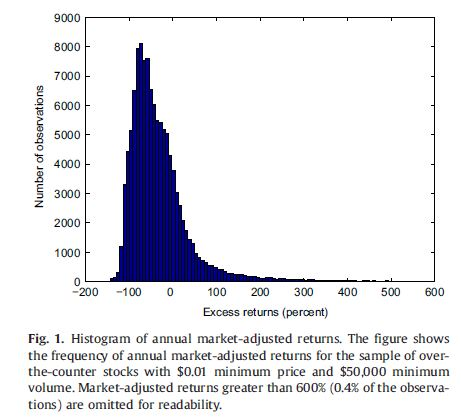
\includegraphics[width=\textwidth]{figures/slide24_pic1.jpg}\\[0.2em]
\footnotesize Eraker and Ready (2015)
\end{column}
\end{columns}
\end{frame}

% --- Slide 25: Under-diversification ---
\begin{frame}[shrink=5]{The Cross-Section, ctd.}
\textbf{Applications, ctd.}
\begin{itemize}
\item Under-diversification
  \begin{itemize}
  \item Mitton and Vorkink (2007) find that under-diversified individuals hold stocks that are more positively skewed than the average stock
  \end{itemize}
\item Several papers test the model's basic prediction that skewness is priced in the cross-section
  \begin{itemize}
  \item The empirical challenge is that past skewness is not a good measure of expected future skewness
  \item Boyer, Mitton, and Vorkink (2010) use a regression model to predict expected skewness using stock characteristics
  \item Bali, Cakici, and Whitelaw (2011) look at maximum daily returns
  \item Conrad, Dittmar, and Ghysels (2013) use option prices to infer the perceived skewness of the underlying stock
  \end{itemize}
\item All three studies find supportive evidence
\end{itemize}
\end{frame}

% --- Slide 26: MAX measure ---
\begin{frame}{Maximum Daily Returns as the Lottery Measure}
\begin{itemize}
\item Bali, Cakici, and Whitelaw (2011) construct a very simple measure of lottery-like features for individual stocks
\item \textbf{MAX:} maximum daily return over the past one month
\item MAX exhibits strong negative return predictability and helps resolve the idiosyncratic volatility puzzle
\end{itemize}
\vfill
\centering
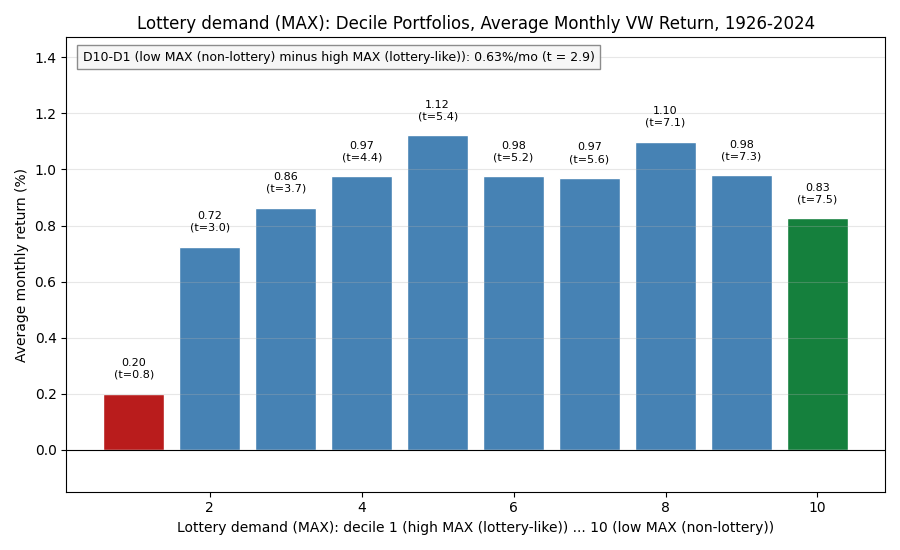
\includegraphics[width=0.45\textwidth]{figures/MaxRet_decile_bar.png}
\end{frame}

% --- Slide 27: Lottery Preference Evidence ---
\begin{frame}[shrink=5]{Evidence Supporting Investor Lottery Preference}
\begin{columns}[T]
\begin{column}{0.50\textwidth}
\begin{itemize}
\item Kumar (2009) shows that the demand for lottery-type stocks is correlated with the demand for lotteries
\item At the aggregate level, individual investors prefer stocks with lottery features
\item The demand for lottery-type stocks increases during economic downturns
\item Socioeconomic factors that induce greater lottery expenditure are associated with greater investment in lottery-type stocks
\item Lottery investment levels are higher in regions with favorable lottery environments
\end{itemize}
\end{column}
\begin{column}{0.46\textwidth}
\centering
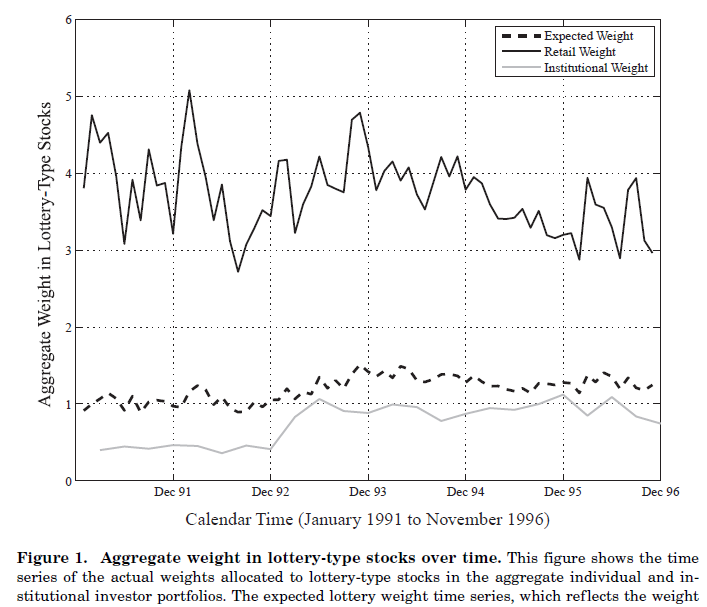
\includegraphics[width=\textwidth]{figures/slide27_pic1.png}
\end{column}
\end{columns}
\end{frame}

% --- Slide 28: Lottery Preference Evidence, ctd. ---
\begin{frame}[shrink=5]{Evidence Supporting Investor Lottery Preference, ctd.}
\begin{itemize}
\item Chen, Hwang, and Peng (RFS 2025) examine why investors like short-leg securities using textual analysis and test whether the justifications primarily (1) emphasize safe-haven qualities, (2) indicate exuberance, or (3) highlight lottery-like features
\end{itemize}
\vfill
\centering
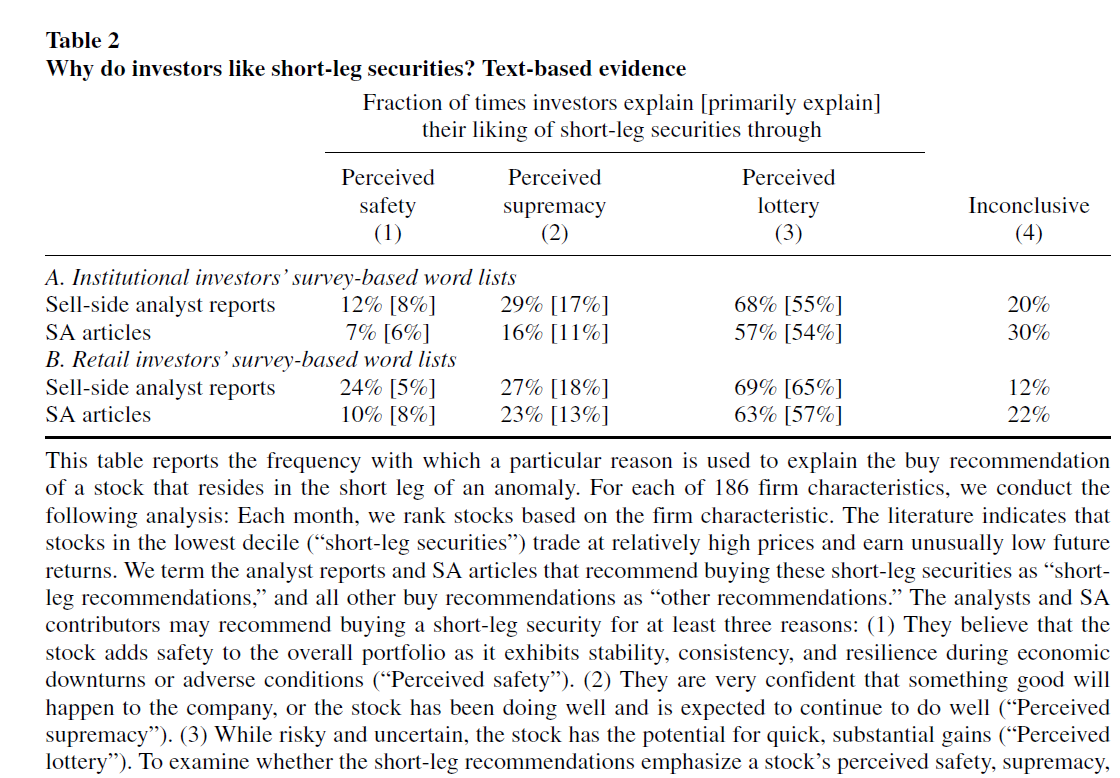
\includegraphics[width=0.65\textwidth]{figures/slide28_pic1.png}
\end{frame}

% --- Slide 29: Model Implications ---
\begin{frame}{The Cross-Section, ctd.}
\begin{itemize}
\item This only works if the security is highly skewed
  \begin{itemize}
  \item Otherwise, an investor would need an excessively undiversified position in order to add skewness to the portfolio
  \end{itemize}
\item \textbf{Note:}
  \begin{itemize}
  \item An example of how psychology can lead to interesting new predictions
  \item Probability weighting plays a central role
  \item The model generates both a low premium on positively skewed stocks and a high premium on the aggregate market
    \begin{itemize}
    \item Because the aggregate market is negatively skewed
    \end{itemize}
  \end{itemize}
\end{itemize}
\end{frame}

% --- Slide 30: Risk-Return Trade-off ---
\begin{frame}[shrink=5]{The Cross-Section, ctd.}
\begin{columns}[T]
\begin{column}{0.50\textwidth}
\begin{itemize}
\item Prospect theory: investors are risk averse over gains, and risk seeking over losses
\item This may help explain the high-risk--low-alpha puzzle
\item Wang, Yan, and Yu (JFE, 2016):
  \begin{itemize}
  \item Following Grinblatt and Han (2005), first construct the stock-level capital gains overhang (CGO), which simply proxies for whether investors collectively have a capital gain on this stock
  \item The cross-sectional risk-return trade-off is positive among stocks in which investors face prior gains
  \item But becomes negative among stocks in which investors face prior losses
  \end{itemize}
\end{itemize}
\end{column}
\begin{column}{0.46\textwidth}
\centering
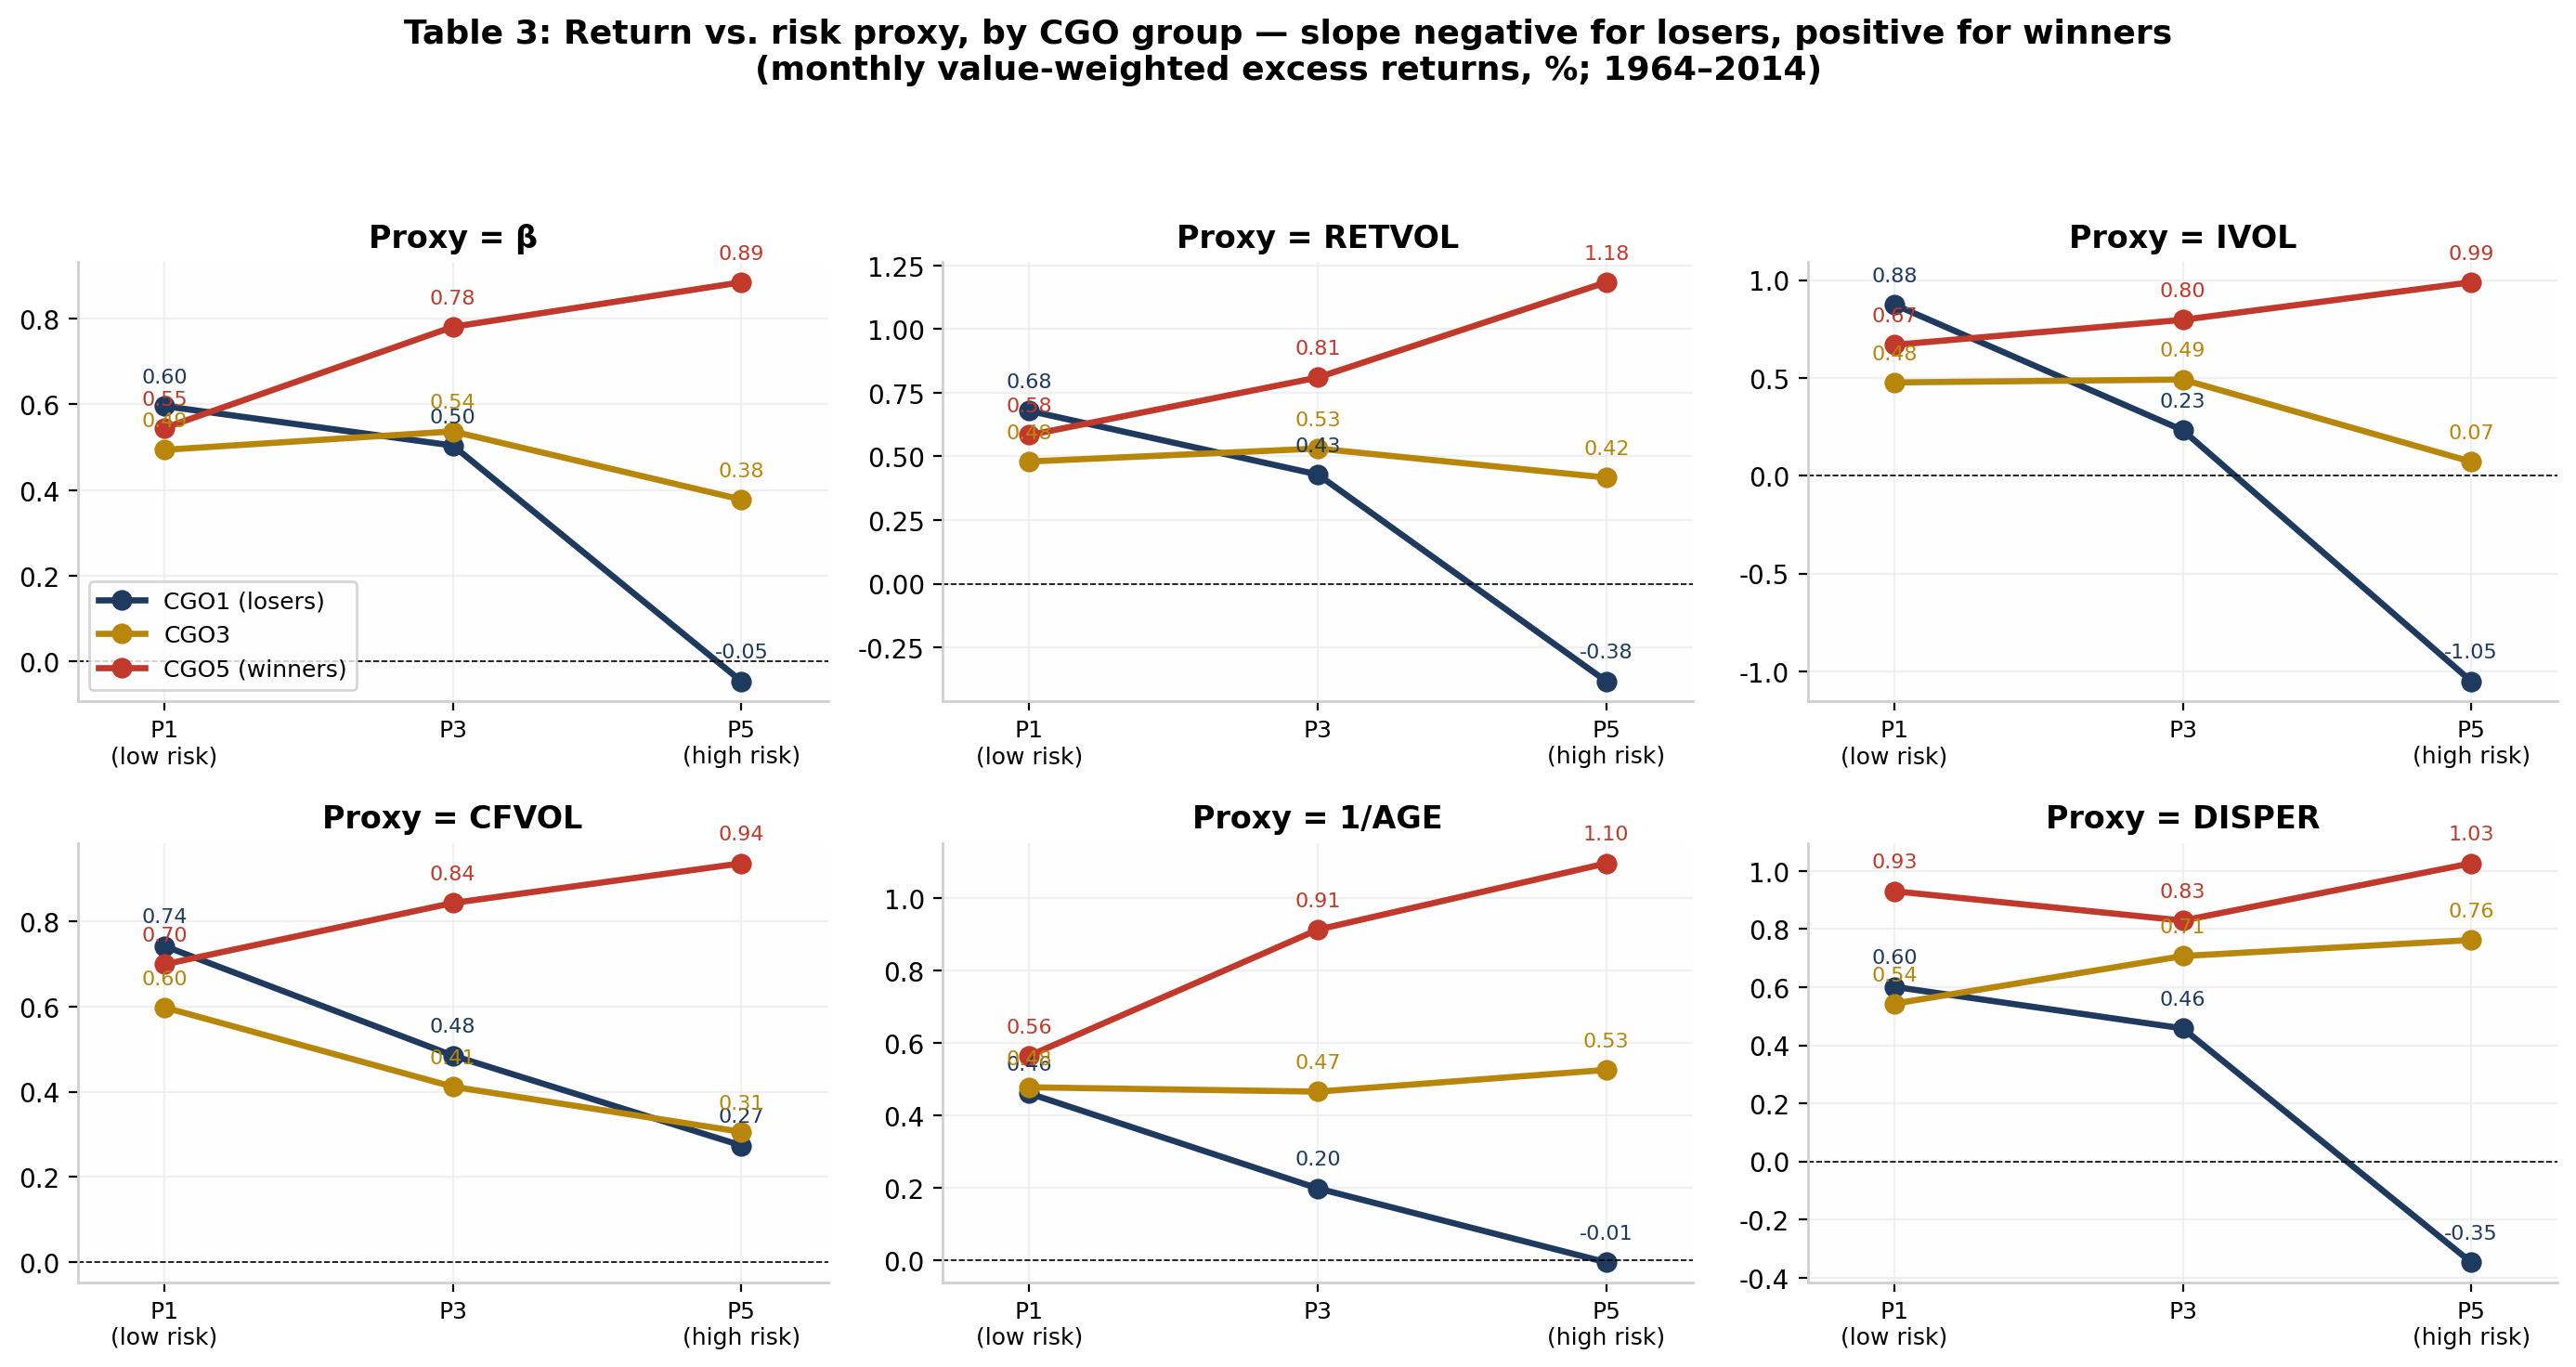
\includegraphics[width=\textwidth]{figures/Table3_return_vs_risk_by_CGO.png}
\end{column}
\end{columns}
\end{frame}

% --- Slide 31: Disposition Effect and Momentum ---
\begin{frame}[shrink=5]{The Cross-Section, ctd.}
\textbf{Applications, ctd.}
\begin{itemize}
\item If many investors display the disposition effect, there will be underreaction to news
  \begin{itemize}
  \item Grinblatt and Han (2005): Momentum; Frazzini (2006): PEAD
  \end{itemize}
\item When a stock experiences good news and increases in value relative to the purchase price, investors want to sell it to lock in the gain, which depresses its price and leads to higher subsequent returns
\item When bad news is released and the price goes down relative to the purchase price, disposition investors are reluctant to sell, leading to underreaction and lower future return
\end{itemize}
\vfill
\centering
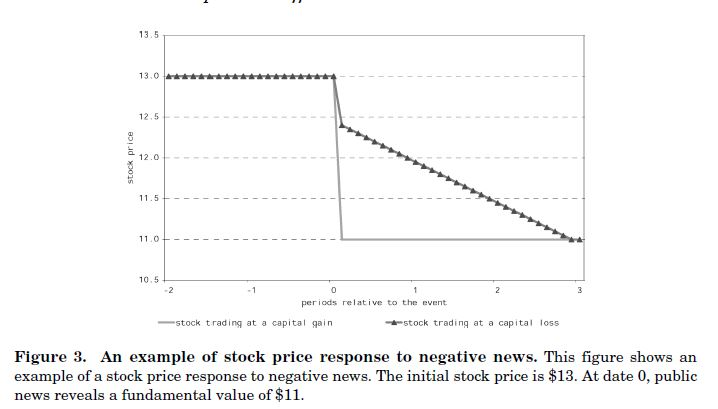
\includegraphics[width=0.42\textwidth]{figures/slide31_pic1.jpg}
\hspace{0.2em}
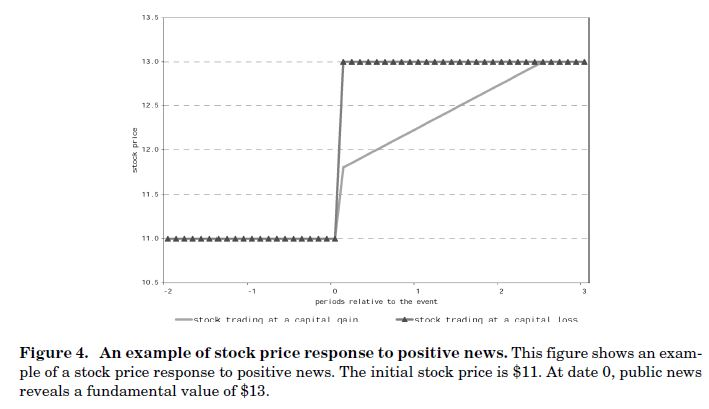
\includegraphics[width=0.42\textwidth]{figures/slide31_pic2.jpg}
\end{frame}

% --- Slide 32: Direct Test ---
\begin{frame}[shrink=5]{Direct Test of Prospect Theory in the Cross-Section}
\textbf{Barberis, Mukerjee, and Wang (RFS 2016):}
\begin{itemize}
\item Investors evaluate the attractiveness of individual stocks based on prospect theory
\item They compute the prospect theory value for each stock using its historical return distribution
\item Stocks with high prospect theory values are more appealing to investors
\item Investors tilt toward these stocks, causing the stocks to become overvalued and to earn lower subsequent returns
\end{itemize}
\vfill
\centering
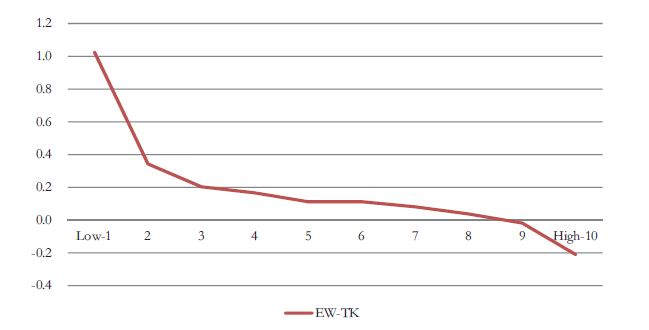
\includegraphics[width=0.55\textwidth]{figures/slide32_pic1.jpg}
\end{frame}

% --- Slide 33: BJW 2021 ---
\begin{frame}{Prospect Theory and Stock Market Anomalies}
\begin{columns}[T]
\begin{column}{0.50\textwidth}
\textbf{Barberis, Jin, and Wang (JF 2021):}
\begin{itemize}
\item Use prospect theory to make quantitative predictions about an asset's average return
\item Based on empirical estimates of the asset's return volatility, return skewness, and past capital gain
\item Compare the model-predicted alphas with actual alphas of anomaly-sorted decile portfolios
\end{itemize}
\end{column}
\begin{column}{0.47\textwidth}
\centering
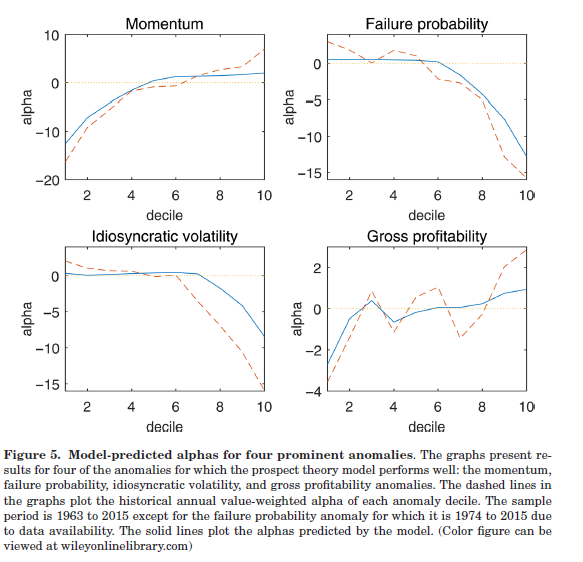
\includegraphics[width=\textwidth]{figures/slide33_pic1.png}
\end{column}
\end{columns}
\end{frame}

% --- Slide 34: BJW 2021, ctd. ---
\begin{frame}{Prospect Theory and Stock Market Anomalies, ctd.}
\begin{columns}[T]
\begin{column}{0.50\textwidth}
\begin{itemize}
\item However, the model performs poorly on the size, value, long-term reversal, short-term reversal, accrual, asset growth, and investment anomalies
\end{itemize}
\end{column}
\begin{column}{0.47\textwidth}
\centering
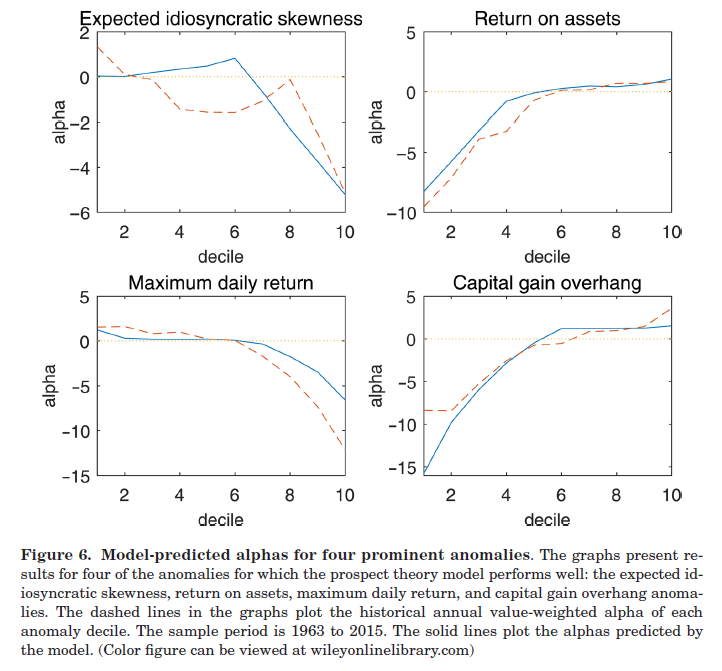
\includegraphics[width=\textwidth]{figures/slide34_pic1.png}
\end{column}
\end{columns}
\end{frame}

% --- Slide 35: Mutual Fund Flows ---
\begin{frame}{Prospect Theory: Revealed Preferences from Mutual Fund Flows}
\begin{itemize}
\item Previous studies mainly test the asset pricing implications of prospect theory
\item But prospect theory also makes predictions about investor demand for certain assets
\item Han, Sui, and Yang (JFE 2026) evaluate prospect theory using mutual fund flows, which directly reveal investor preference/demand across assets
\item They document that funds whose past returns generate higher prospect theory value attract significantly larger future flows
\end{itemize}
\end{frame}


% --- Slide 35a: Instructor's research ---
\begin{frame}[shrink=5]{My Research: Stock Splits as Behavioral Signals}
	\begin{itemize}
		\item \textbf{Li, Cui, Pang, and Xie (Financial Management, forthcoming)}
		\begin{itemize}
			\item We try to explain why stock splits can be a credible positive signal to markets, even though the costs of implementing stock splits are trivial 
			\item Model: retail investors are loss averse and treat stock splits as good news
			\item A split raises expectations about future firm fundamentals and price appreciation, while missing those expectations triggers disproportionately large price declines
			\item In equilibrium, only managers with favorable information use splits to signal: loss aversion makes splits credible
			\item Evidence from China: investors turn more optimistic after splits, higher split ratios bring stronger market reactions, and splitting firms' prices fall harder when they miss elevated expectations
		\end{itemize}
		\item \textbf{Connection:} an application of loss aversion (this lecture) to corporate events: splits work as signals \emph{because} investors evaluate outcomes as gains and losses relative to an elevated reference point
	\end{itemize}
\end{frame}

% --- Slide 36: Aggregate Stock Market ---
\section{The Aggregate Stock Market}

\begin{frame}[shrink=5]{The Aggregate Stock Market}
\begin{itemize}
\item Can prospect theory help us understand the properties of, and attitudes to, the aggregate stock market?
  \begin{itemize}
  \item Benartzi and Thaler (1995) note that a model in which investors are loss averse over annual changes in the value of their stock market holdings predicts a large equity premium
  \item Three elements:
    \begin{itemize}
    \item Loss aversion
    \item Annual evaluation of gain and loss (why?)
    \item Narrow framing
    \end{itemize}
  \item Benartzi and Thaler (1995) emphasize the first two elements -- ``myopic loss aversion''
  \end{itemize}
\end{itemize}
\end{frame}

% --- Slide 37: Benartzi and Thaler ---
\begin{frame}[shrink=5]{The Aggregate Stock Market, ctd.}
\textbf{Benartzi and Thaler (1995):}
\begin{itemize}
\item The prospect theory value of the historical distribution of annual US stock market returns is approximately equal to the prospect theory value of the historical distribution of annual US bond market returns
\item On the one hand, the greater volatility of stock market returns serves to lower its prospect theory value relative to that of bond market returns
\item On the other hand, the much higher average return of the stock market serves to increase the prospect theory value of the stock market
\item Benartzi and Thaler (1995) show that these two forces cancel out
\item The stock market earns a high average return so that it can be competitive with the bond market in the eyes of prospect theory investors
\end{itemize}
\end{frame}

% --- Slide 38: Graph ---
\begin{frame}{The Aggregate Stock Market, ctd.}
\vfill
\centering
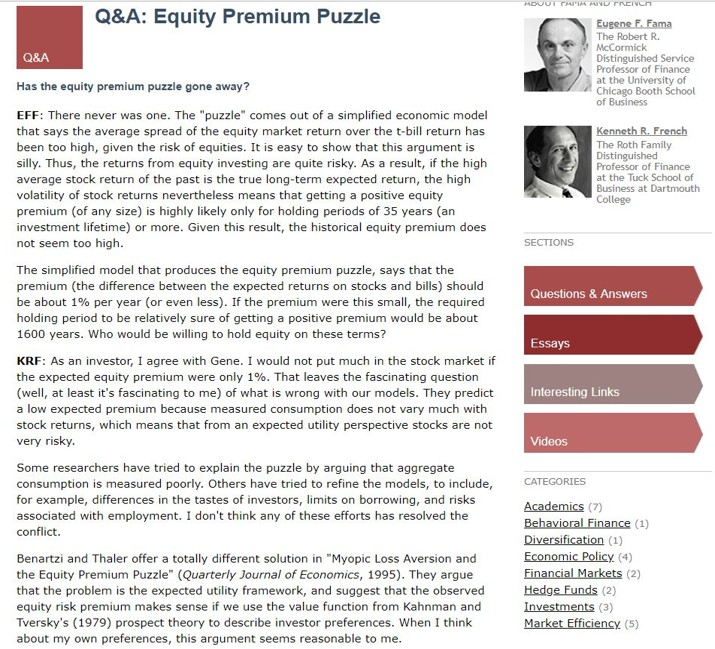
\includegraphics[width=0.50\textwidth]{figures/38.jpg}
\end{frame}

% --- Slide 39: Role of Narrow Framing ---
\begin{frame}[shrink=5]{The Aggregate Stock Market, ctd.}
\textbf{The role of narrow framing}
\begin{itemize}
\item Barberis, Huang, and Santos (2001) find that narrow framing is a critical ingredient
  \begin{itemize}
  \item Loss aversion over total wealth fluctuations does not produce a significant equity premium
  \item Nor will it generate non-participation in the stock market
  \item The stock market has low correlation with other risks
  \end{itemize}
\end{itemize}
\vspace{0.5em}
\textbf{The role of probability weighting}
\begin{itemize}
\item De Giorgi and Legg (2012) introduce probability weighting and show that it can significantly increase the equity premium
  \begin{itemize}
  \item Because the aggregate stock market is negatively skewed: it is subject to occasional large crashes
  \item Under probability weighting, investors overweight this left-tail outcome, which makes the stock market even less appealing
  \end{itemize}
\end{itemize}
\end{frame}

% --- Slide 40: Ambiguity Aversion ---
\section{Ambiguity Aversion}

\begin{frame}[shrink=5]{Ambiguity Aversion}
\begin{itemize}
\item Economists have long distinguished between ``risk'' and ``uncertainty''
  \begin{itemize}
  \item Risk: the decision-maker is able to assign probabilities to the various possible outcomes
  \item Uncertainty: not able to assign probabilities to these outcomes
  \end{itemize}
\item \textbf{The Ellsberg paradox, 1961}
\item Two urns:
  \begin{itemize}
  \item Urn C: 100 balls, 50 Red, 50 Black
  \item Urn U: 100 balls, either Red or Black, unknown distribution
  \end{itemize}
\item Choose between:
  \begin{itemize}
  \item Bet R1: draw a ball from urn C, get \$100 if Red
  \item Bet R2: draw a ball from urn U, get \$100 if Red
  \end{itemize}
\item Choose between:
  \begin{itemize}
  \item Bet B1: draw a ball from urn C, get \$100 if Black
  \item Bet B2: draw a ball from urn U, get \$100 if Black
  \end{itemize}
\item The modal participant chooses both R1 and B1, suggesting that people act as if Urn C contains more red balls and more black balls than Urn U
\end{itemize}
\end{frame}

% --- Slide 41: Ambiguity Aversion Applications ---
\begin{frame}[shrink=5]{Ambiguity Aversion: Applications}
\begin{itemize}
\item Ambiguity aversion has been applied in finance in a number of ways (Epstein and Schneider, 2010).
\item \textbf{Non-participation:}
  \begin{itemize}
  \item The return on the stock market is more ambiguous than the return on a bank deposit or on Treasury Bills (Dow and Werlang, 1992)
  \end{itemize}
\item \textbf{Equity premium puzzle:}
  \begin{itemize}
  \item If investors are ambiguity averse, they will require a much higher average return on the stock market than on Treasury Bills (Maenhout, 2004)
  \end{itemize}
\item \textbf{Under-diversification:}
  \begin{itemize}
  \item Individuals view the returns of the domestic stock market, locally-headquartered stocks, and their own company stock as less ambiguous than foreign stock markets, distant stocks, and non-company stocks, respectively (Uppal and Wang, 2003)
  \end{itemize}
\end{itemize}
\end{frame}

\end{document}
